% !TeX root = ../thesis.tex

\chapter{Data Representation}
\label{sec:data_representation}

This chapter presents description about data representations. Since panoptic task requires to learn both modalities i.e. semantic segmentation and instance segmentation, it also demands the ground-truth label data to be presented in a suitable format for either modalities. First section of this chapter discusses semantic ground-truth representation and dataset used for this purpose. Second section is dedicated to the description of various instance representations and encodings that are conceived and generated during the course of this master thesis.  




\section{Semantic Label Representation}

This section describes about the dataset used for experiments, more specifically this section gives a brief overview of semantic segmentation labels used for this purpose. 

\paragraph{Cityscapes}

Cityscapes is a large-scale benchmark dataset that contains diverse street scenes from 50 different cities, with a high quality pixel-level and instance-level semantic labeling annotations of 5000 frames at resolution of $1024 \times 2048$ in addition to a larger set of 20000 coarsely annotated frames \cite{Cordts2015}. Cityscapes has become a default benchmark for semantic segmentation due to its high quality of annotation along with high resolution labeled images \cite{DBLPbenchmark:journals/corr/abs-1709-07322}. Figure \ref{fig:cityscapes} illustrates
some example segmentation annotations from cityscapes dataset overlaid on corresponding RGB image captured in different cities. Furthermore, fine-annotations are further divided into 3 splits, which is an important step carried out for learning process. One split is used for learning the parameters in an iterative process, while other is used for monitoring models performance during  the training (learning process), the last split is used at the end of learning process to test models performance.

\begin{table}[!htbp]
    \centering
        \begin{tabular}{llll}
        \hline \bigskip & \multicolumn{3}{c} {Cityscapes } \\
        \cline { 2 - 4 } Dataset split & $\mathrm{CS}_{\text {train }}$ & $\mathrm{CS}_{\text {val }}$ & $\mathrm{CS}_{\text {test }}$ \\
        \hline Number of images  & 2975 & 500 & 1500 \\
        \hline
        \end{tabular}
    \caption[Data Splits in Cityscapes]{Training, validation and test splits of Cityscapes.}
    \label{tab:cityscapessplits}
\end{table}



\begin{figure}[!ht]
        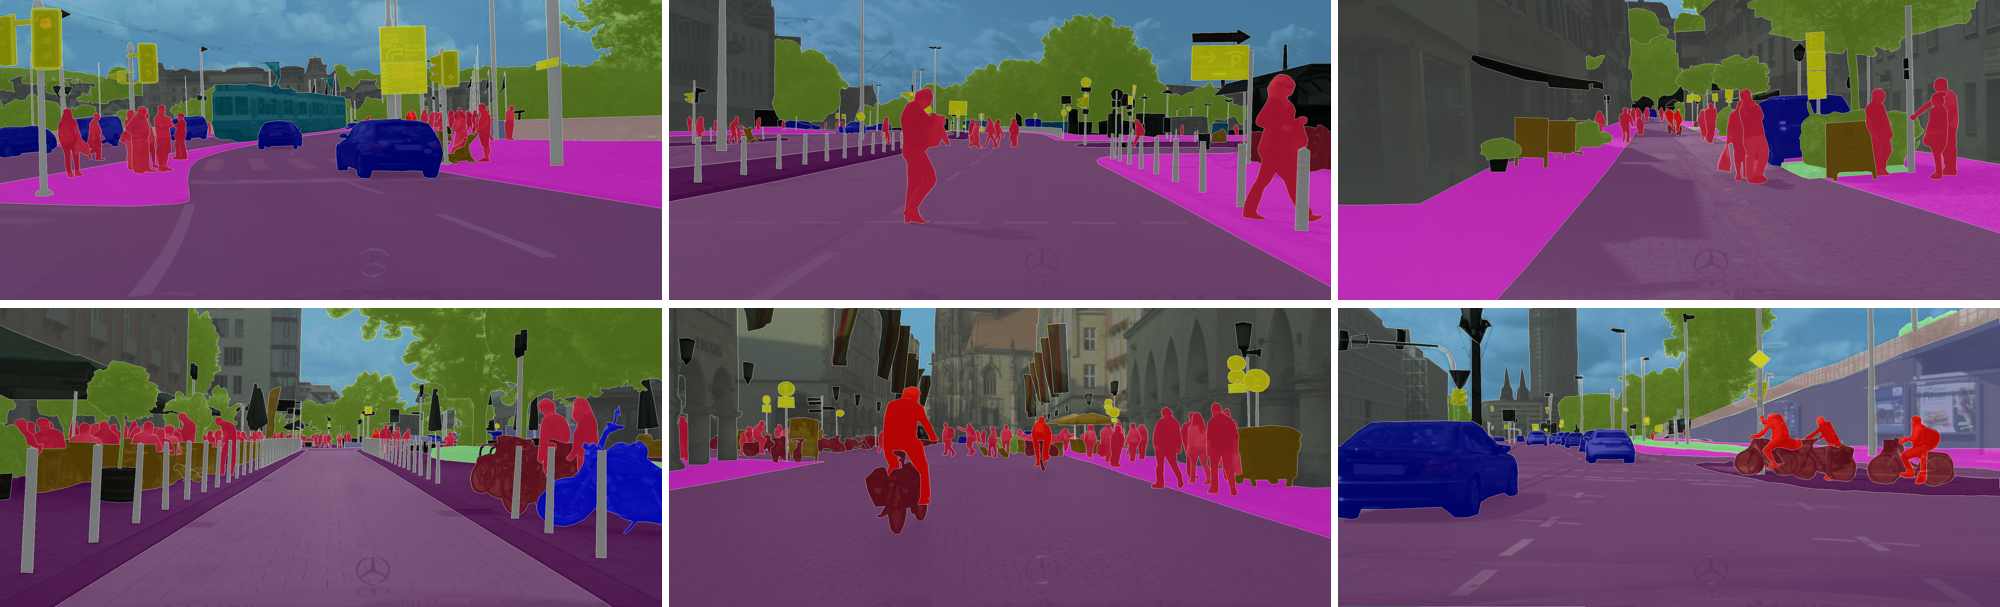
\includegraphics[width = \textwidth]{Graphics/Data_Representation/cityscapessamples.png}
    \caption[Examples from Cityscapes dataset]{Illustration of sample images overlayed with corresponding semantic annotations taken from cityscapes dataset \cite{Cordts2015}}
    \label{fig:cityscapes}
\end{figure}


\newpage
\begin{itemize}
    \item \textbf{Train} - split used to train model for optimizing parameters
    \item \textbf{Validation} - split used to monitor model performance during learning
    \item \textbf{Test} - split used to evaluate performance of trained model at the end of learning process.
\end{itemize}

Training labels for semantic segmentation are used directly as provided by cityscapes. The groundtruth is annotated to distinguish 31 different classes, however they are usually summarized to 19 classes for training purposes which have also been used within the scope of this thesis as such.

\section{Instance Representation}

One core objective of the presented work is to learn pixel-level relationships for instance segmentation instead of using $2-stage$ objection detection like architecture for instance segmentation. This section is dedicated to describe the instance representations for encoding instance information which is later learned by the network in combination with semantic segmentation. The following section illustrates instance representations that are conceived during the scope of this thesis. A general approach adapted to represent pixel relationships is to encode the distance for every pixel within an instance to its corresponding center point. Firstly, the representation and encoding center point information is discussed. Subsequently, various offset representations are discussed that in some way describe the offset of every pixels from its respective center. 


\subsection{Center Points Representation}

It is desire
d to learn instance representations in addition to semantic segmentation of the scene. To generate an instance representation, center point for every instance is considered to be a reference point. Therefore it is critical that this reference representation is robust and efficiently learned by the network. To locate a center from an instance annotation, distance transform is employed to binary mask of individual instance  \cite{Borgefors1986} -  see chapter \ref{sec:fundamentals}. In addition to being robust against heavy occlusions, this also has the benefit of being a consistent approach for locating center of visible portion of instances appearing in an image. In computer vision literature, it is common to denote key points by encoding them with a 2d - gaussian distribution \cite{DBLPCPM:journals/corr/WeiRKS16}, \cite{Bulat2016HumanPE}. Center points extracted from every instance mask are therefore encoded by a probability distribution around the center. A visualisation of such center rendering and encoding each center with a 2d - gaussian like distribution has been shown in the figure \ref{fig:centerpoints} 

\begin{figure}[!ht]
    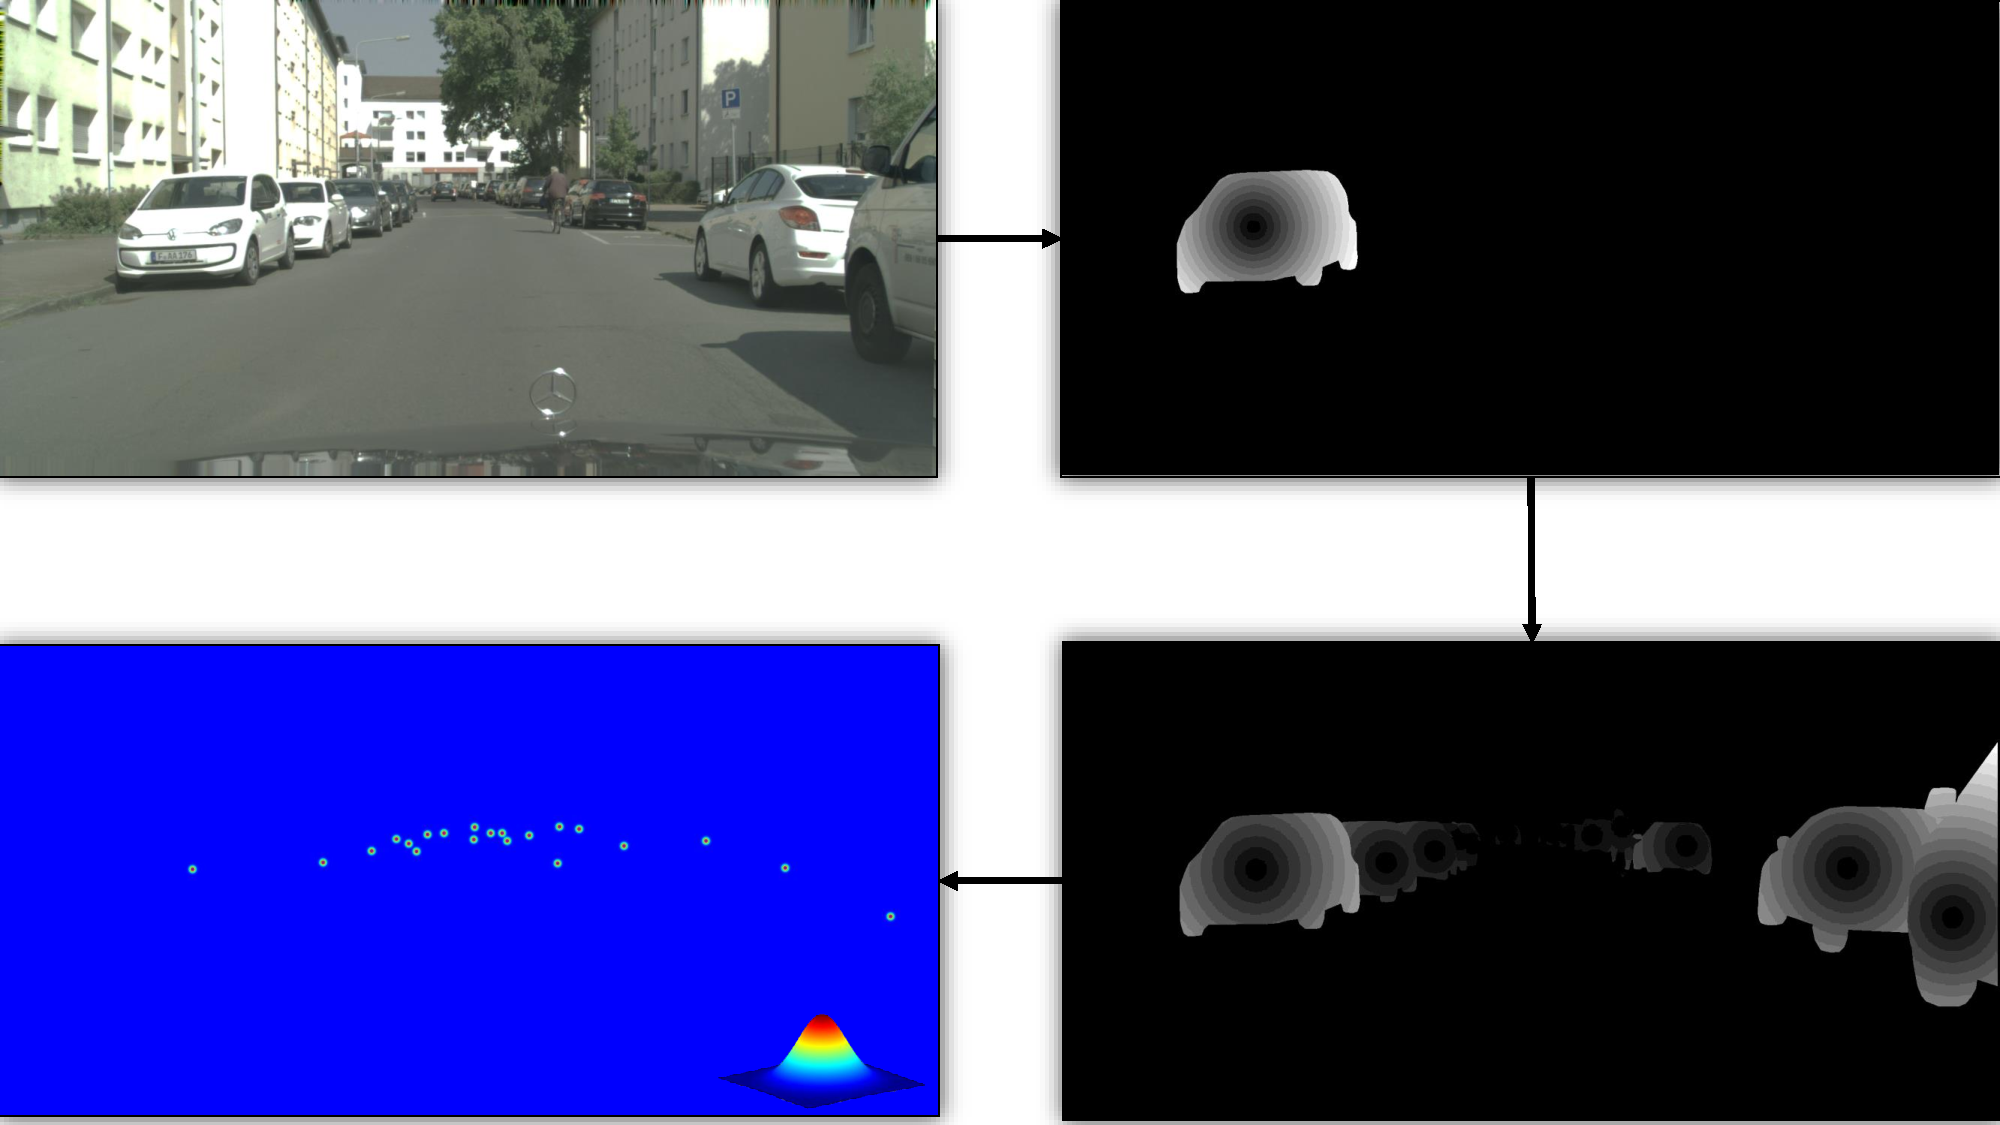
\includegraphics[width = \textwidth]{Graphics/Data_Representation/dist_centerpoints.pdf}
    \caption[Center Encoding Process]{Illustration of center encoding process. Distance transformation is applied to every instance and pixel with largest distance to the boundary is selected to be the center for each instance. Subsequently, each center point is encoded with a 2d - gaussian distribution.}
    \label{fig:centerpoints}
\end{figure}

It has also been shown that representing a key-point with a gaussian distribution comparatively improves performance, such experiments have also been carried out by \cite{Cheng_2020_CVPR}, they also show that an additional $0.8\%$ improvement can be made if such an encoding is used and optimized using L2 -loss between predicted and ground-truth label instead of categorical cross-entropy (which is a commonly employed loss function for semantic segmentation problems in image domain). 

However, the right size for this purpose is still an open question. If a center point is encoded with a probability distribution of very small standard deviation ($\sigma$) , it might not considerably influence the learning process, since every image has a high resolution of 1024 $\times$ 2048, on the other hand if the $\sigma$ is too large, it might be very dispersed around center point region (thus not representing precise location of center point) and might also pose a problem of overlapping nearby center points. Hence it is desired to generate datasets with center-points encoded as gaussians of variable standard deviations $\sigma$ and compare the performance to reason about the right distribution parameters. For this purpose, 4 datasets have been generated that encode center-points with different $\sigma$, which in this case are chosen to be 2, 4, 8 and 16, see figure \ref{fig:distsizes}. The results for which have been discussed in evaluation chapter.

\begin{figure}[!ht]
    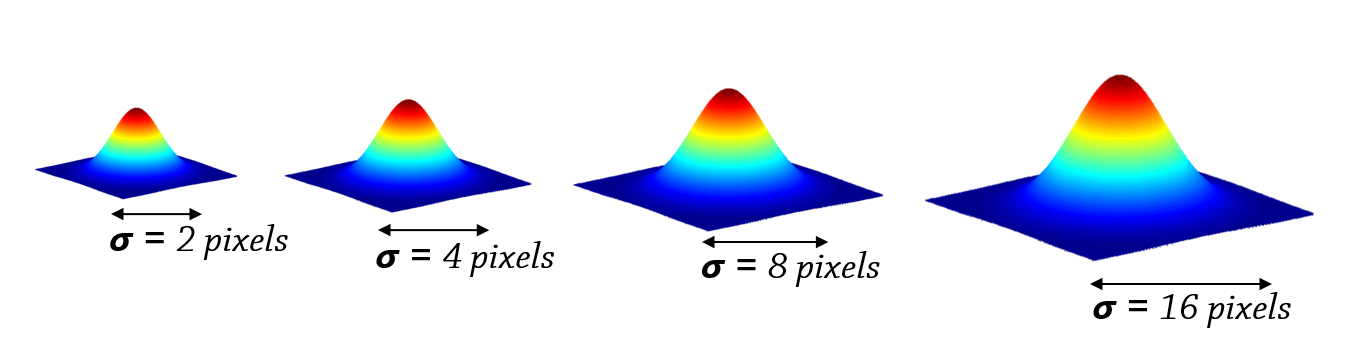
\includegraphics[width = \textwidth]{Graphics/Data_Representation/distributions}
    \caption[Different Distribution Sizes]{Visualisation of different guassian distributions with variable  standard deviations of  2, 4, 8 and 16 - from left to right respectively.}
    \label{fig:distsizes}
\end{figure}



\subsection{Offset Representation}

\label{subsec:offsets}
Another important information that has been used to encode instances is\textit{ offset vectors}. Offset vector representation can be elaborated as - a representation where every \textit{thing} class pixel encodes the distance to its corresponding center hence, the \textit{offset which when added to the pixel at given location will move it to its corresponding center.} Few such offset vector representations that have been generated and evaluated during this work are named as follows:

\begin{enumerate}

    \item End-to-end encoding
    \item Center-to-end encoding 
    \item Euclidean encoding

\end{enumerate}

Visualisation of the above mentioned offset vector encodings has been shown as rgb images in the figure \ref{fig:RGB_encodings}. These representations will be explained in detail in the following sub-sections.

\begin{figure}[!ht]
%\centering
        \subfigure[Center-to-End Encoding]{
        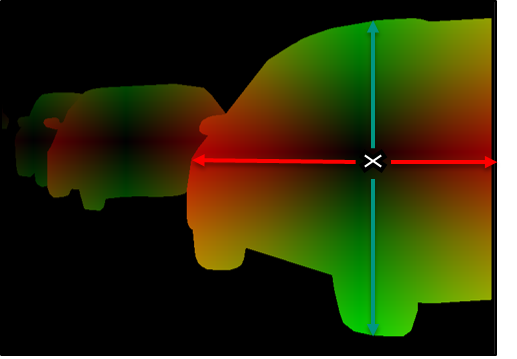
\includegraphics[width = \textwidth / 3 ]{Graphics/Data_Representation/c2e_vis_img}
        \label{fig:c2e_img_vis}}\subfigure[End-to-End Encoding]{
        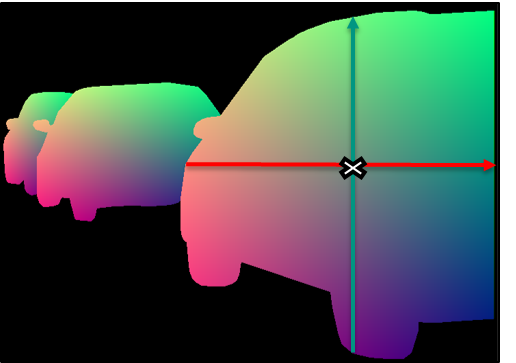
\includegraphics[width = \textwidth / 3 ]{Graphics/Data_Representation/e2e_vis_img}
        \label{fig:e2e_img_vis}}\subfigure[Euclidean Encoding]{
        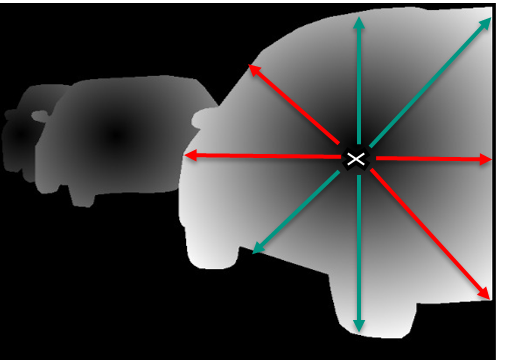
\includegraphics[width = \textwidth / 3 ]{Graphics/Data_Representation/euc_vis_img}
        \label{fig:euc_img_vis}}
        \caption[RGB Visualisation of Offset Vectors Encoding]{Visualisations of conceived encodings as rgb images a) center to end encoding b) end to end Encoding c) euclidean encoding}
        \label{fig:RGB_encodings}
\end{figure}

\subsubsection{End to End Encoding}
\label{subsec:e2e}
One way to encode aforementioned offset is by encoding both distance and direction information at given pixel location. The value encoded by each pixels exhibits a positive or a negative distance to the center point depending on it's relative position with respect to center. Additionally, the offset in horizontal axis and vertical axis are encoded independently i.e. one channel is used to record the offset in x-axis and another channel records the offset in y-axis. This can be understood by a simple case in horizontal direction, where pixels on the left side to the center will have a positive distance to the center - representing a positive offset needed to reach to the center and pixel on the right side relative to center would exhibit a negative offset - representing a negative offset needed to reach the center point.  Encoding offsets in such a way yield a near perfect representation where each pixel can be re-assigned to one of given centers at hand.  
\begin{figure}[!ht]
    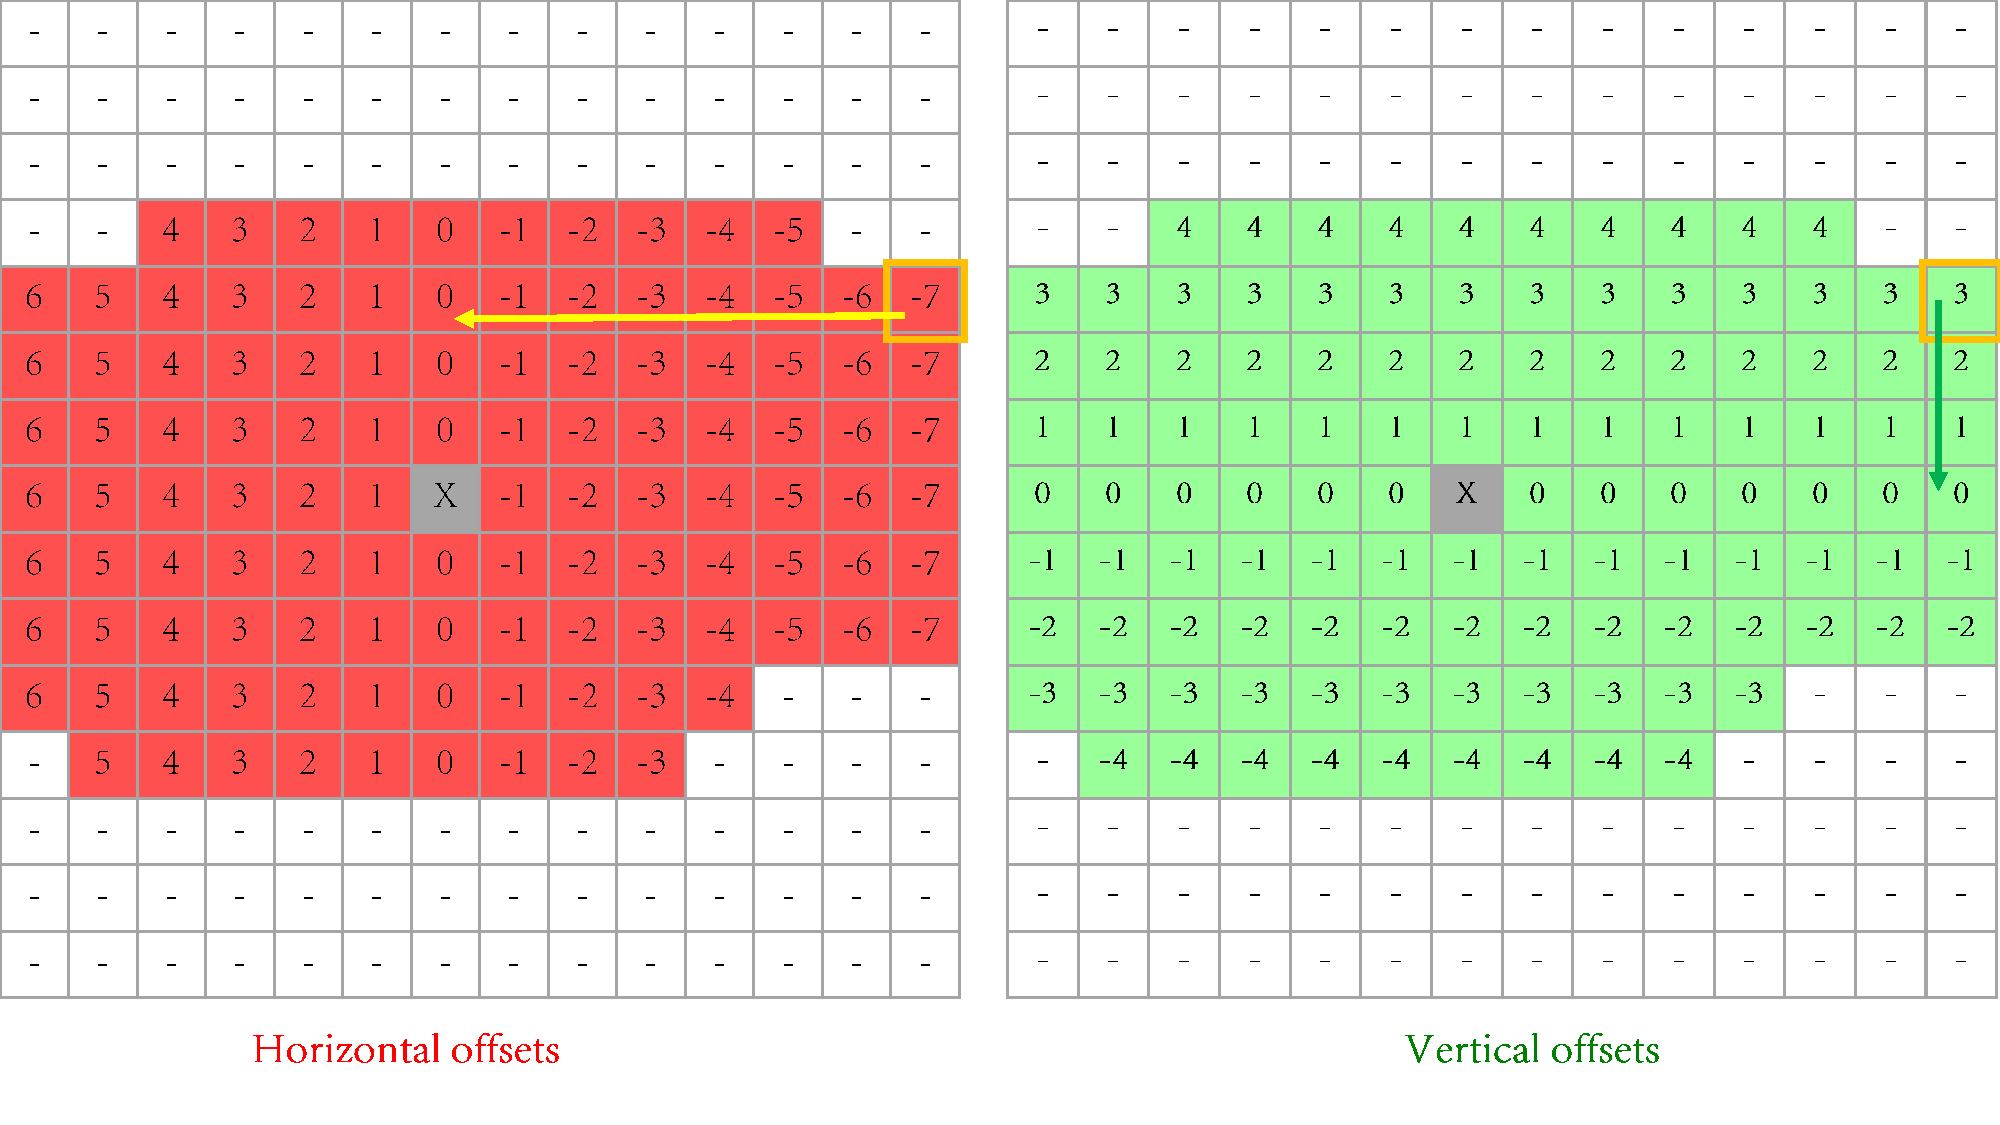
\includegraphics[width = \textwidth]{Graphics/Data_Representation/c2e_Encoding.pdf}
    \caption[Center to End Encoding]{Illustration of End-to-End encoding}
    \label{fig:e2e_vis_pixels}

\end{figure}

Once, the offset in horizontal and vertical axis $o(i, j)$ is extracted for a given pixel at location $(i, j)$, from both channels, these offsets can be added to the pixel location yielding the location of the center  $C_{k}$ of instance that pixel belongs to. Illustration of such an offset vectors representation has been shown in the figure \ref{fig:e2e_vis_pixels}. 

It can be seen from figure \ref{fig:e2e_vis_pixels}, that pixels on right side of center point are encoded as negative offsets in horizontal offset representation. Similarly, pixels below center point are encoded as negative offsets in vertical offset representation. Hence explicitly defining the direction as well as magnitude needed to reach center point. Such representation which one learned would just require a simple regression to group pixels with their corresponding centers. Another observation that can be made from this representation is the fact that offset values increase on one side of the center while decrease on the other side of the center hence a representation where offset values increase linearly between either ends of the instance. Therefore it has been named as \textit{End-to-End Encoding}. See figure \ref{fig:e2e_plt_vis} for reference.

\subsubsection{Center to End Encoding}
\label{subsec:c2e}
Another possibility to encode offset is encoding only distance information irrespective of direction towards the center at given pixel location. 

Since, direction information is not considered explicitly, it might appear as if encoding such offset representation would result in ambiguity while recovering the instances by regressing pixels to their centers. However, it can be shown that this is not the case. The offset vector therefore always exhibit positive distance to the center point irrespective of position with respect to center.  Here as well, the offsets in horizontal axis and vertical axis are encoded independently i.e. one channel is used to record the offset in x-axis and another channel records offset in y-axis. 
As, direction information is not explicitly encoded, it then requires additional post-processing step by inverting the offset values on one side in both horizontal and vertical offset representations. Theoretically, if network learns to predict as good as original groundtruth labels, it would result in a very adequate re-assignment of all the pixels to one of the centers. 

Once,  the offset vectors are inverted to re-construct offset vectors with direction information,  offset  in  horizontal  and  vertical  axis $o(i,j)$  is  extracted  for  a  given  pixel  at location $(i,j)$, from both channels, these offsets can be added to the pixel location $(i,j)$ yielding the center $C_{k}$ of instance that pixel belongs to. Illustration of such an offset vectors representation has been shown in the figure \ref{fig:c2e_vis_flip}. It can be seen the representation has taken the form of the previous end to end offset, which would then again employ a simple regression to group pixels with their corresponding centers.
Offset values appear to increase on either sides of the center point hence a representation where offset values increase monotonically on either side of center point of an instance. Therefore  it has  been named as center-to-end encoding. See figure \ref{fig:c2e_plt_vis} for reference.


\begin{figure}[!ht]
%\centering
        \subfigure[Center-to-End Encoding]{
        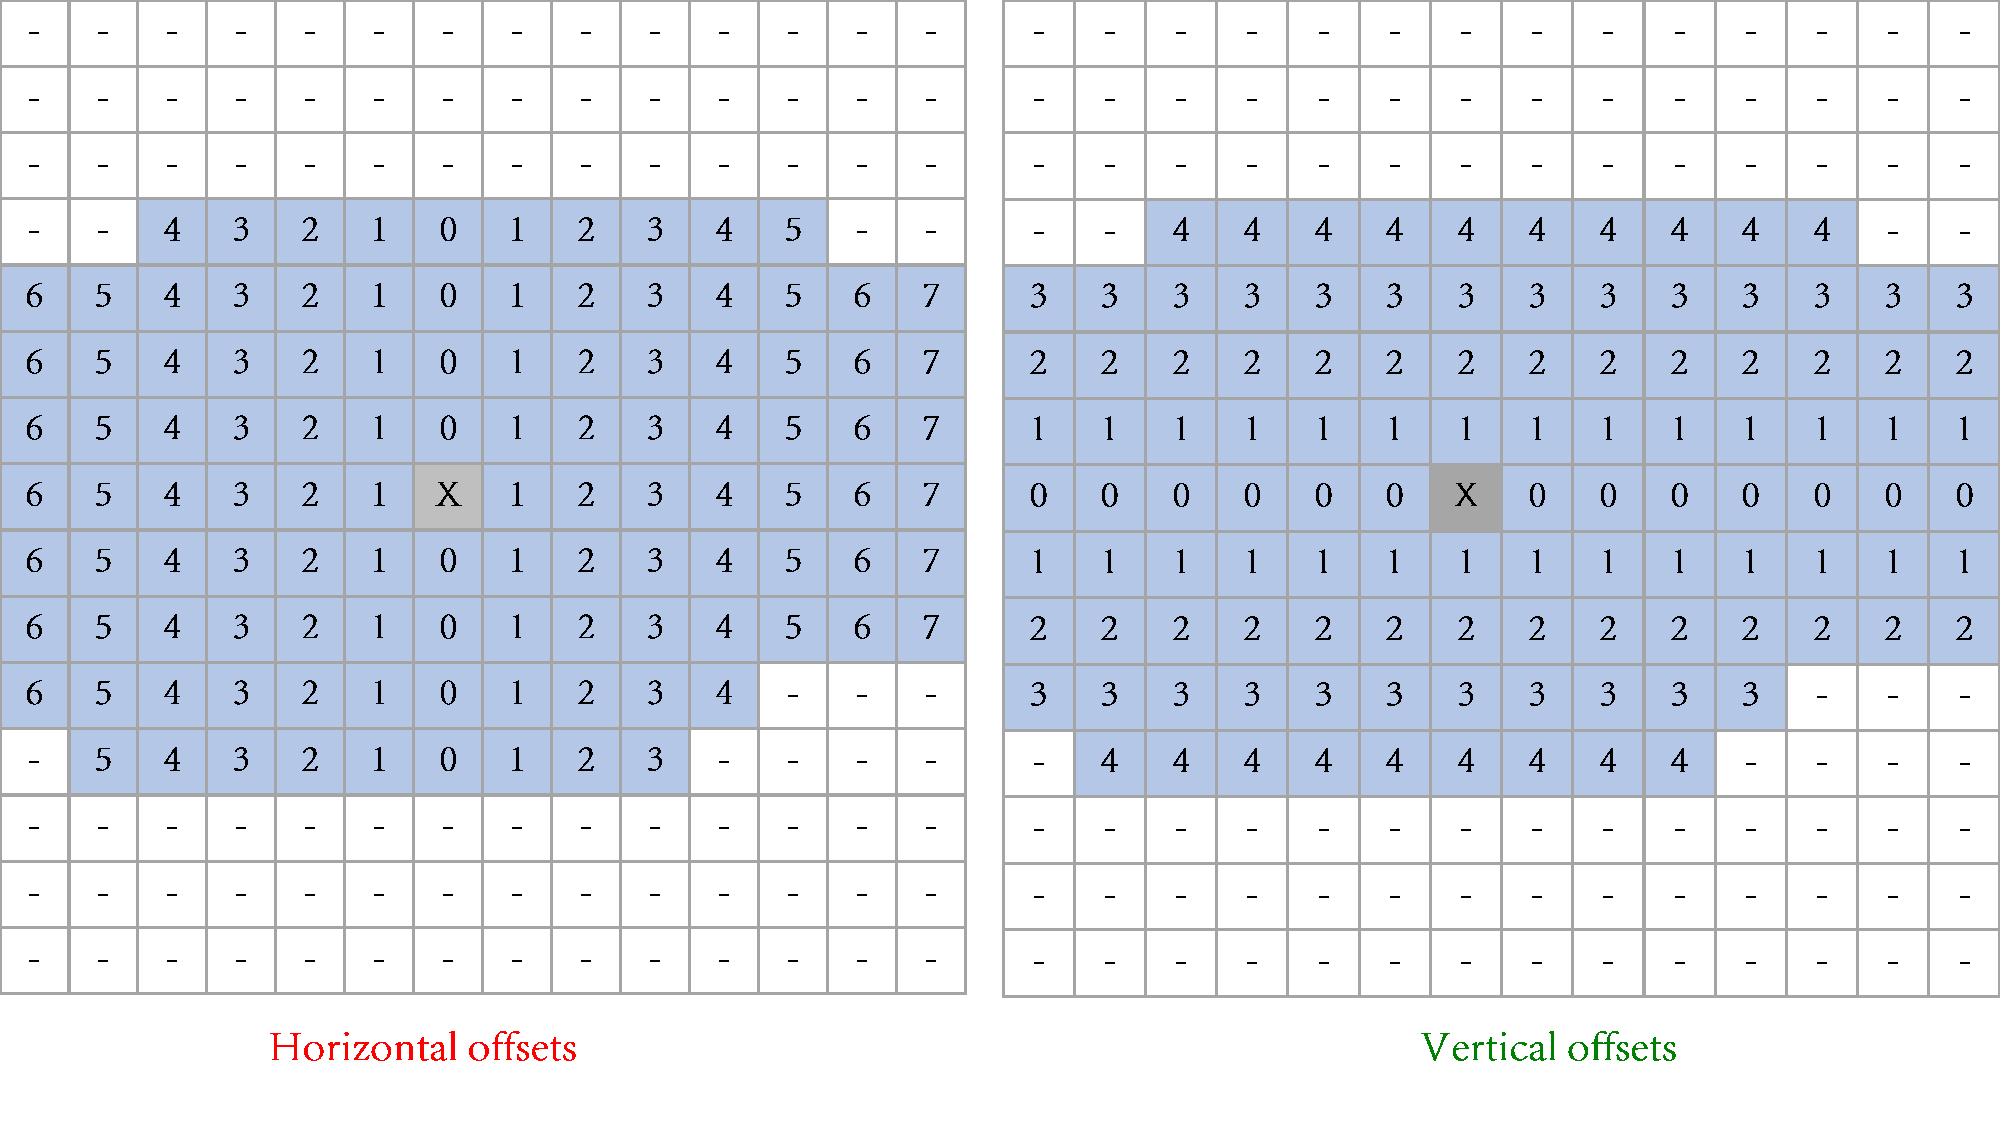
\includegraphics[width = \textwidth]{Graphics/Data_Representation/c2e_vis}
        \label{fig:c2e_vis}}
        
        \subfigure[Center-to-End Encoding Inverted]{
        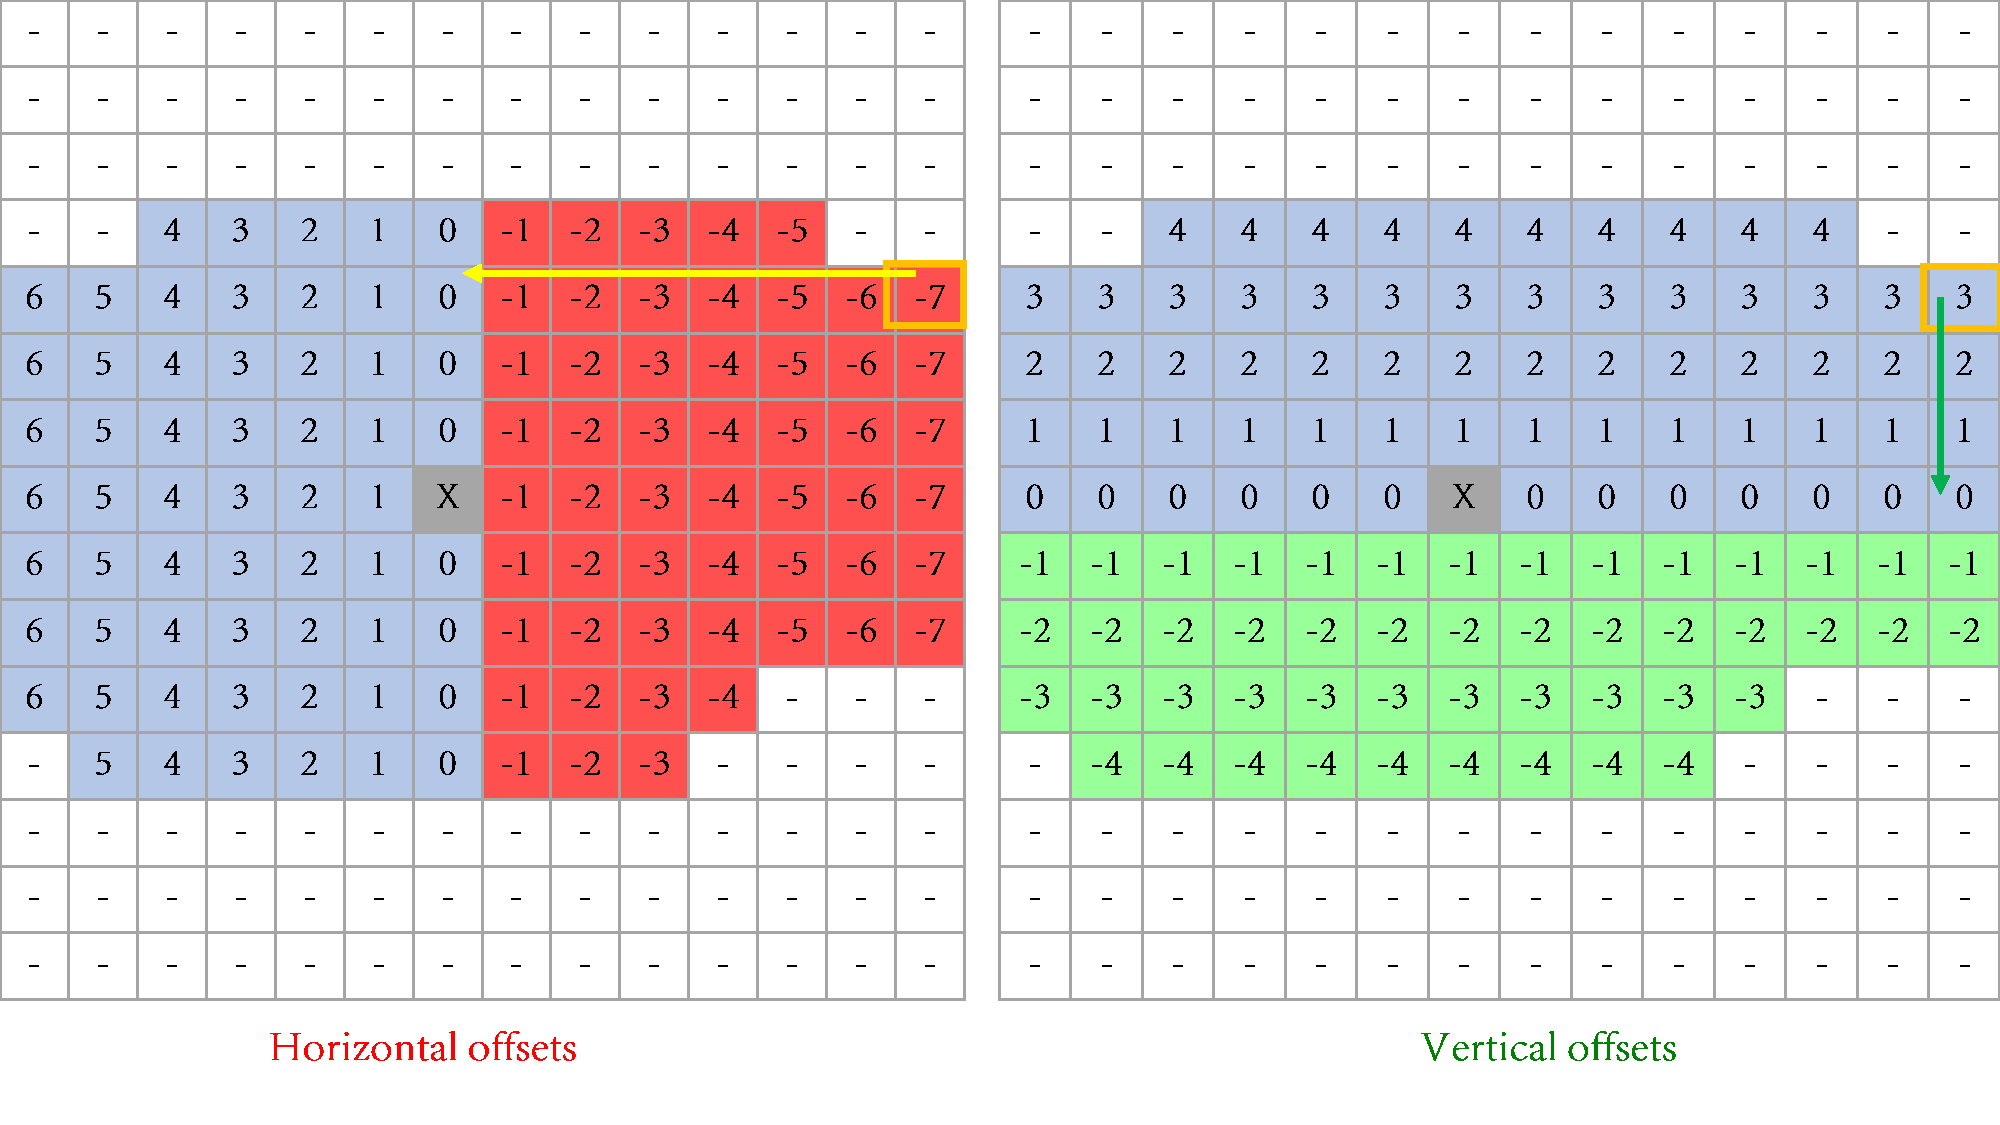
\includegraphics[width = \textwidth]{Graphics/Data_Representation/c2e_vis_flipped}
        \label{fig:c2e_vis_flip}}
        \caption[Center to End Encoding with Direction Recovering] {Illustration of center-to-end encoding and direction recovering a) shows a center-to-end encoding b) shows the offset directions recovered by inverting the offset values in center-to-end encoding}
        \label{fig:c2e_vis_pixels}
\end{figure}



\subsubsection{Euclidean Encoding}

Another way of encoding offset vectors is encoding euclidean distance. Given a pixel position, euclidean distance to corresponding instance center point is calculated and encoded at the same pixel location.  In such a representation, the direction is not considered at all as encoded value is calculated as a euclidean distance between given pixel position $(i,j)$ and corresponding center point $C_{k}(x_{1}, y_{1})$. This information can then be directly encoded in a single channel. Although a simple representation, it may not be the most effective and would also require an additional computational overhead by explicitly projecting each pixel to the direction of each center point in an image for calculating the distance between pixel position and center. Therefore, resulting in a single channel offset representation for generating groundtruth labels but is more ambiguous and demands extra computational expense. Visualisation of such representation can be seen in the figure \ref{fig:euc_img_vis}.

\begin{figure}[!ht]
%\centering
        \subfigure[End-to-End Encoding]{
        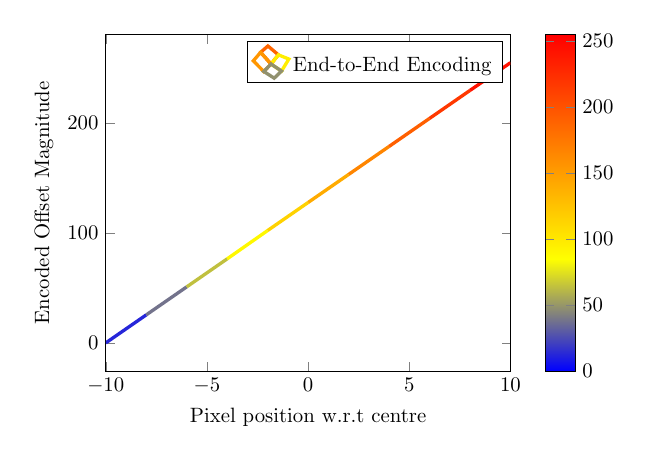
\begin{tikzpicture}[every axis/.style={
                xmax=10,%
                xmin=-10,%
                ylabel={Encoded Offset Magnitude },%
                xlabel={Pixel position w.r.t centre },%
                ytick={}
                }, scale=0.75]
                	\begin{axis}[colorbar]
                		\addplot[mesh, ultra thick,  width= \textwidth /2 ]         
                		plot coordinates { 
                            (-10, 0)
                            (-8, 25.5)
                            (-6, 51)
                            (-4, 76.5)
                            (-2, 102.3)
                            (0, 127.8)
                            (2, 153.3)
                            (4, 178.8)
                            (6, 204.3)
                            (8, 229.8)
                            (10, 255)
                        };;
                        \addlegendentry{ End-to-End Encoding}
                	\end{axis}
                \end{tikzpicture}
        \label{fig:e2e_plt_vis}}
        \subfigure[Center-to-End Encoding]{
        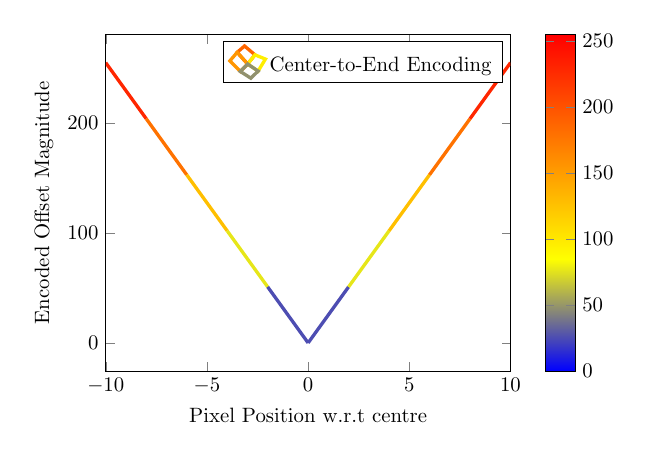
\begin{tikzpicture}[every axis/.style={
                xmax=10,%
                xmin=-10,%
                ylabel={Encoded Offset Magnitude},%
                xlabel={Pixel Position w.r.t centre },%
                ytick={}
                }, scale=0.75]
                	\begin{axis}[colorbar]
                
                		\addplot[mesh, ultra thick]         
                		plot coordinates {
                            (-10,255)
                            (-8,204)
                            (-6,153)
                            (-4,102)
                            (-2,51)
                            (0,0)
                            (2,51)
                            (4,102)
                            (6,153)
                            (8,204)
                            (10,255)
                        };;
                          \addlegendentry{Center-to-End Encoding}
                	\end{axis}
                \end{tikzpicture}
        \label{fig:c2e_plt_vis}}
            \caption[Plots representing Encoded Values]{Plots representing encoded value patterns a) shows end-to-end encoding where offset values increases linearly between either ends b) shows plot for center-to-end encoding where value increases monotonically in either directions around center point.}
    \label{fig:encodings_plots}
\end{figure}

















